% =============================================================================
% Project : THE_PHILOSOPHY_OF_VIABILITY
% Book    : Book I — Ontology of Viability
% Book ID : VS.B01
%
% File    : 4_ASSETS/diagrams/
%           VS.B01.P01.C03.S04.SS06.P003.DG01.identity_plurality_across_ontological_levels.tex
%
% Asset   : DG01 — Identity Plurality Across Ontological Levels
%
% Purpose :
%   To display distinct levels at which unity and plurality
%   may be asserted, without implying a necessary hierarchy
%   or numerical correspondence among them.
%
% =============================================================================

\begin{figure}[htbp]
\centering

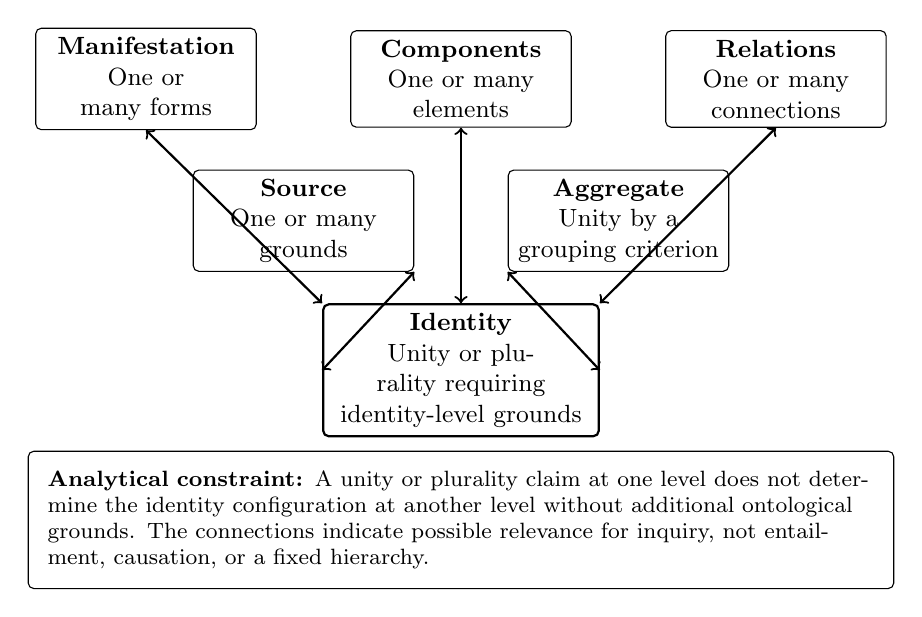
\begin{tikzpicture}[
    levelbox/.style={
        draw,
        rounded corners=2pt,
        align=center,
        minimum width=2.8cm,
        minimum height=0.95cm,
        text width=2.55cm,
        font=\small
    },
    identitybox/.style={
        draw,
        rounded corners=2pt,
        thick,
        align=center,
        minimum width=3.5cm,
        minimum height=1.15cm,
        text width=3.2cm,
        font=\small
    },
    relation/.style={
        <->,
        thick
    },
    note/.style={
        draw,
        rounded corners=2pt,
        align=left,
        text width=10.5cm,
        inner sep=7pt,
        font=\footnotesize
    }
]

\node[levelbox] (manifestation) at (-4.0,1.6) {
    \textbf{Manifestation}\\
    One or many forms
};

\node[levelbox] (components) at (0,1.6) {
    \textbf{Components}\\
    One or many elements
};

\node[levelbox] (relations) at (4.0,1.6) {
    \textbf{Relations}\\
    One or many connections
};

\node[levelbox] (source) at (-2.0,-0.2) {
    \textbf{Source}\\
    One or many grounds
};

\node[levelbox] (aggregate) at (2.0,-0.2) {
    \textbf{Aggregate}\\
    Unity by a grouping criterion
};

\node[identitybox] (identity) at (0,-2.1) {
    \textbf{Identity}\\
    Unity or plurality requiring
    identity-level grounds
};

\draw[relation] (manifestation.south) -- (identity.north west);
\draw[relation] (components.south) -- (identity.north);
\draw[relation] (relations.south) -- (identity.north east);
\draw[relation] (source.south east) -- (identity.west);
\draw[relation] (aggregate.south west) -- (identity.east);

\node[note] at (0,-4.0) {
    \textbf{Analytical constraint:}
    A unity or plurality claim at one level does not determine
    the identity configuration at another level without
    additional ontological grounds. The connections indicate
    possible relevance for inquiry, not entailment, causation,
    or a fixed hierarchy.
};

\end{tikzpicture}

\caption{Distinct ontological levels relevant to the analysis of identity plurality}
\label{fig:identity-plurality-across-ontological-levels}

\end{figure}

% =============================================================================
% END OF ASSET DG01
% =============================================================================